\documentclass[conference]{IEEEtran}
\IEEEoverridecommandlockouts
% The preceding line is only needed to identify funding in the first footnote. If that is unneeded, please comment it out.
%Template version as of 6/27/2024

\usepackage{cite}
\usepackage{amsmath,amssymb,amsfonts}
\usepackage{algorithmic}
\usepackage{graphicx}
\usepackage{textcomp}
\usepackage{xcolor}
\def\BibTeX{{\rm B\kern-.05em{\sc i\kern-.025em b}\kern-.08em
    T\kern-.1667em\lower.7ex\hbox{E}\kern-.125emX}}
\begin{document}

\title{Chinese Chess HCI Robot\\}

\author{
	\IEEEauthorblockN{Shengzhe Gan}
	\IEEEauthorblockA{
		Dept. of EEE, SUSTech\\
		Shenzhen, China \\
		12313107@mail.sustech.edu.cn}
	\and
	\IEEEauthorblockN{Yugong Wang}
	\IEEEauthorblockA{
		Dept. of EEE, SUSTech\\
		Shenzhen, China \\
		12312820@mail.sustech.edu.cn}
	\and
	\IEEEauthorblockN{Yihan Wang}
	\IEEEauthorblockA{
		Dept. of EEE, SUSTech\\
		Shenzhen, China \\
		12310811@mail.sustech.edu.cn}
}


\maketitle

\begin{abstract}
This project presents the development of a Chinese Chess Human-Computer Interaction (HCI) robot, which integrates advanced robotics, computer vision, and AI techniques to create an interactive chess-playing system. The robot utilizes the Robot Operating System (ROS) for real-time communication and navigation, powered by an Intel RealSense D435 camera and a KINOVA Gen3 Lite robotic arm. The key features include dynamic chessboard recognition using YOLOv8s for object detection, precise motion planning with forward and inverse kinematics, and a chess-playing AI based on Minimax and Alpha-Beta pruning algorithms. The system is capable of recognizing the chessboard layout and identifying piece positions, enabling the robot to play Chinese Chess interactively. The project explores the integration of visual recognition, motion control, and AI decision-making, providing a foundation for future developments in educational, entertainment, and research applications. Future work will focus on enhancing the accuracy of chessboard recognition, optimizing the robotic arm's movement strategies, and improving overall system stability.
\end{abstract}

\begin{IEEEkeywords}
Motion Planning,Forward and Inverse Kinematics,Object Detection,Robotic Manipulation,Computer Vision.
\end{IEEEkeywords}

\section{Introduction}
Human-Computer Interaction (HCI) has become a crucial area in robotics research, combining artificial intelligence, computer vision, and control theory to create systems capable of interacting with humans in dynamic environments. Board games like Chinese Chess provide an ideal platform to explore these interactions, offering both structured rules and complex spatial reasoning. Compared to virtual agents, physical HCI systems pose a unique challenge: they must perceive the environment accurately, make intelligent decisions, and execute motions within the mechanical and dynamic limits of the robot hardware.

In this project, we present a real-world Chinese Chess HCI robot system that integrates a 6-DoF Kinova Gen3 Lite manipulator with an Intel RealSense D435 depth camera, controlled via the Robot Operating System (ROS). The robot autonomously detects the chessboard and pieces using a YOLOv8-based vision module, interprets the current game state, and computes optimal moves using a rule-based AI engine based on Minimax and Alpha-Beta pruning. The entire process—from visual recognition to physical interaction—is executed in a closed-loop system, enabling the robot to play chess in real time against a human opponent.

A core technical challenge in such a system lies in the precise and reliable control of the manipulator. To address this, we design and implement two distinct motion control strategies:

\begin{itemize}
	\item \textbf{API-based control:} This method utilizes Kinova's Kortex API for trajectory planning, relying on calibrated coordinate transforms and forward kinematics to generate high-level motion commands.
	\item \textbf{Algorithmic control:} To achieve finer control and greater flexibility, we implement an inverse kinematics solver combined with time-parameterized cubic polynomial trajectory interpolation. This approach allows explicit modeling of joint velocity and acceleration profiles to ensure smooth and feasible motion.
\end{itemize}

Unlike previous chess-playing robots that typically use planar XY platforms or fixed-position actuators with limited adaptability, our system demonstrates the potential of general-purpose manipulators in dynamic HCI tasks. By integrating real-time perception, decision-making, and compliant motion planning, our work moves towards an intelligent physical agent capable of safe, reliable, and interpretable interaction with humans in shared spaces.


\section{Review}
The integration of robotics, computer vision, and artificial intelligence to create human-interactive chess-playing robots has been an active area of research in recent years \cite{b1}\cite{b4}. The current project builds on this research foundation by developing a Chinese Chess HCI Robot that utilizes a 6-DOF robotic arm and depth camera for physical interactive play.

Several past studies have developed chess-playing robots using robotic arms\cite{b1}\cite{b4}. However, most existing systems rely on custom chessboards or specific computer vision solutions. In contrast, the current project uses a standard Chinese Chessboard and combines it with a generic 6-DOF robotic arm and depth camera. This enables more flexible and precise physical interaction compared to previous systems.

The project also makes several technical contributions:

It uses ROS (Robot Operating System) for modular and distributed system design\cite{b2}.

It implements an optimized inverse kinematics solution and cubic polynomial trajectory generation for precise arm movements \cite{b4}.

It utilizes a custom YOLOv8s convolutional neural network for real-time piece recognition with high accuracy\cite{b3}.

In comparison, previous chess-playing robot systems often used simpler image processing methods for piece recognition\cite{b1}  and less optimized kinematics solutions\cite{b4}. The current project therefore extends the state-of-the-art by integrating more advanced techniques from computer vision and robotics.

In summary, this project builds on past research by developing a more flexible and capable Chinese Chess HCI Robot through the integration of a standard chessboard, generic robotic arm, depth camera, and advanced techniques like ROS, YOLOv8s, and optimized kinematics. Its contributions extend the capabilities of existing chess-playing robots.

\section{Method}

\subsection{System Overview}

The architecture of our Chinese Chess HCI robot is illustrated in Fig.~\ref{fig:system}. The system comprises three main components: a vision module for board detection and recognition, a decision module for move generation, and a motion module that executes robot trajectories via two distinct control strategies. The integration is based on the Robot Operating System (ROS), enabling modular design, real-time communication, and hardware abstraction.

\begin{figure}[htbp]
	\centering
	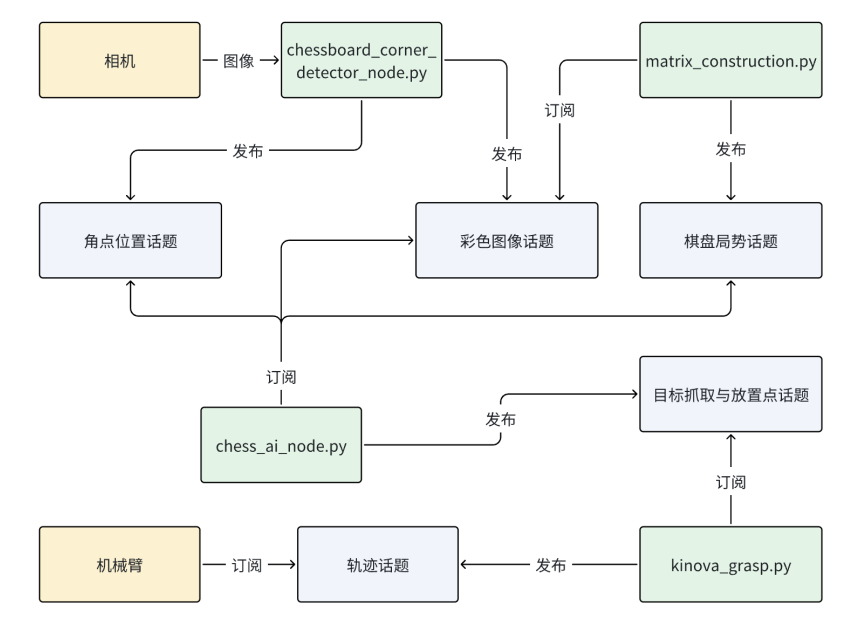
\includegraphics[width=0.45\textwidth]{figures/system_architecture.png}
	\caption{System architecture of the Chinese Chess HCI robot.}
	\label{fig:system}
\end{figure}

\subsection{Visual Perception and Calibration}

We employ YOLOv8 as the backbone of the object detection module to recognize chess pieces and board corners in real time. The model is trained on a custom dataset collected under varied lighting conditions and camera angles. To achieve accurate mapping from image to world coordinates, we conduct camera intrinsic calibration using the standard OpenCV toolbox and estimate the extrinsic transform using a chessboard calibration grid.

The final transformation from the camera frame to the robot base frame is defined as:
\begin{equation}
	\mathbf{T}_{\text{base}}^{\text{cam}} = \mathbf{T}_{\text{base}}^{\text{ee}} \cdot \mathbf{T}_{\text{ee}}^{\text{cam}}
\end{equation}
where $\mathbf{T}_{\text{ee}}^{\text{cam}}$ is measured via hand–eye calibration and $\mathbf{T}_{\text{base}}^{\text{ee}}$ is obtained from forward kinematics.

\subsection{Motion Control}

We design two motion planning strategies for the Kinova Gen3 Lite arm, each suited for different use cases and research flexibility.

\textbf{Strategy 1} utilizes Kinova's built-in trajectory generation API in \texttt{kortex\_driver} \cite{b4}. Given accurate extrinsic parameters of the camera, the end-effector's target pose is transformed to the robot base frame, and the trajectory is generated automatically. The forward kinematics is computed as:
\begin{equation}
	\mathbf{T}_{\text{base}}^{\text{ee}} = \prod_{i=1}^{n} T_i(q_i)
\end{equation}
where $T_i(q_i)$ is the transformation matrix of joint $i$ given its angle $q_i$. This approach ensures high precision due to tightly integrated hardware and reliable calibration.

\textbf{Strategy 2} implements custom inverse kinematics (IK) and cubic polynomial interpolation. The IK is formulated as an optimization problem:
\begin{equation}
	\min_{\mathbf{q}} \; \| f(\mathbf{q}) - \mathbf{T}_{\text{target}} \|
\end{equation}
where $f(\mathbf{q})$ represents the forward kinematics mapping of joint angles $\mathbf{q}$, and $\mathbf{T}_{\text{target}}$ is the desired pose.

To generate smooth motion, we apply cubic polynomial interpolation for each joint. The coefficients $a_0$, $a_1$, $a_2$, and $a_3$ are computed from boundary conditions:
\begin{align}
	a_0 &= \theta_{\text{start}} \\
	a_1 &= v_{\text{start}} \\
	a_0 + a_1 T + a_2 T^2 + a_3 T^3 &= \theta_{\text{end}} \\
	a_1 + 2a_2 T + 3a_3 T^2 &= v_{\text{end}}
\end{align}

The joint position, velocity, and acceleration trajectories are then given by:
\begin{align}
	\Theta(t) &= a_0 + a_1 t + a_2 t^2 + a_3 t^3 \\
	V(t) &= a_1 + 2a_2 t + 3a_3 t^2 \\
	a(t) &= 2a_2 + 6a_3 t
\end{align}

\subsection{Software Communication Architecture}

All modules communicate over ROS topics and services. The vision node publishes object detection results to the decision module, which then sends target poses to the motion node. The decision module maintains an internal representation of the chessboard state and uses a classic game-tree search algorithm to determine optimal moves. Specifically, we implement the Minimax algorithm with Alpha-Beta pruning \cite{b6}, which efficiently evaluates future game states up to a certain depth, enabling the robot to make competitive and rational decisions in real time.

For hardware execution, we use Kinova’s \texttt{kortex\_api} and \texttt{kortex\_driver} ROS packages \cite{b5}, which provide interfaces to send joint trajectories, monitor feedback, and handle low-level motion control. This modular design enables tight coupling between perception, planning, and actuation, essential for responsive human-robot interaction in a dynamic board game environment.



\section{Result}
pass

\section{Discussion}
pass

\section{Conclusion}
\begin{table}[htbp]
	\caption{Table Type Styles}
	\begin{center}
		\begin{tabular}{|c|c|c|c|}
			\hline
			\textbf{Table}&\multicolumn{3}{|c|}{\textbf{Table Column Head}} \\
			\cline{2-4} 
			\textbf{Head} & \textbf{\textit{Table column subhead}}& \textbf{\textit{Subhead}}& \textbf{\textit{Subhead}} \\
			\hline
			copy& More table copy$^{\mathrm{a}}$& &  \\
			\hline
			\multicolumn{4}{l}{$^{\mathrm{a}}$Sample of a Table footnote.}
		\end{tabular}
		\label{tab1}
	\end{center}
\end{table}

\begin{figure}[htbp]
	\centerline{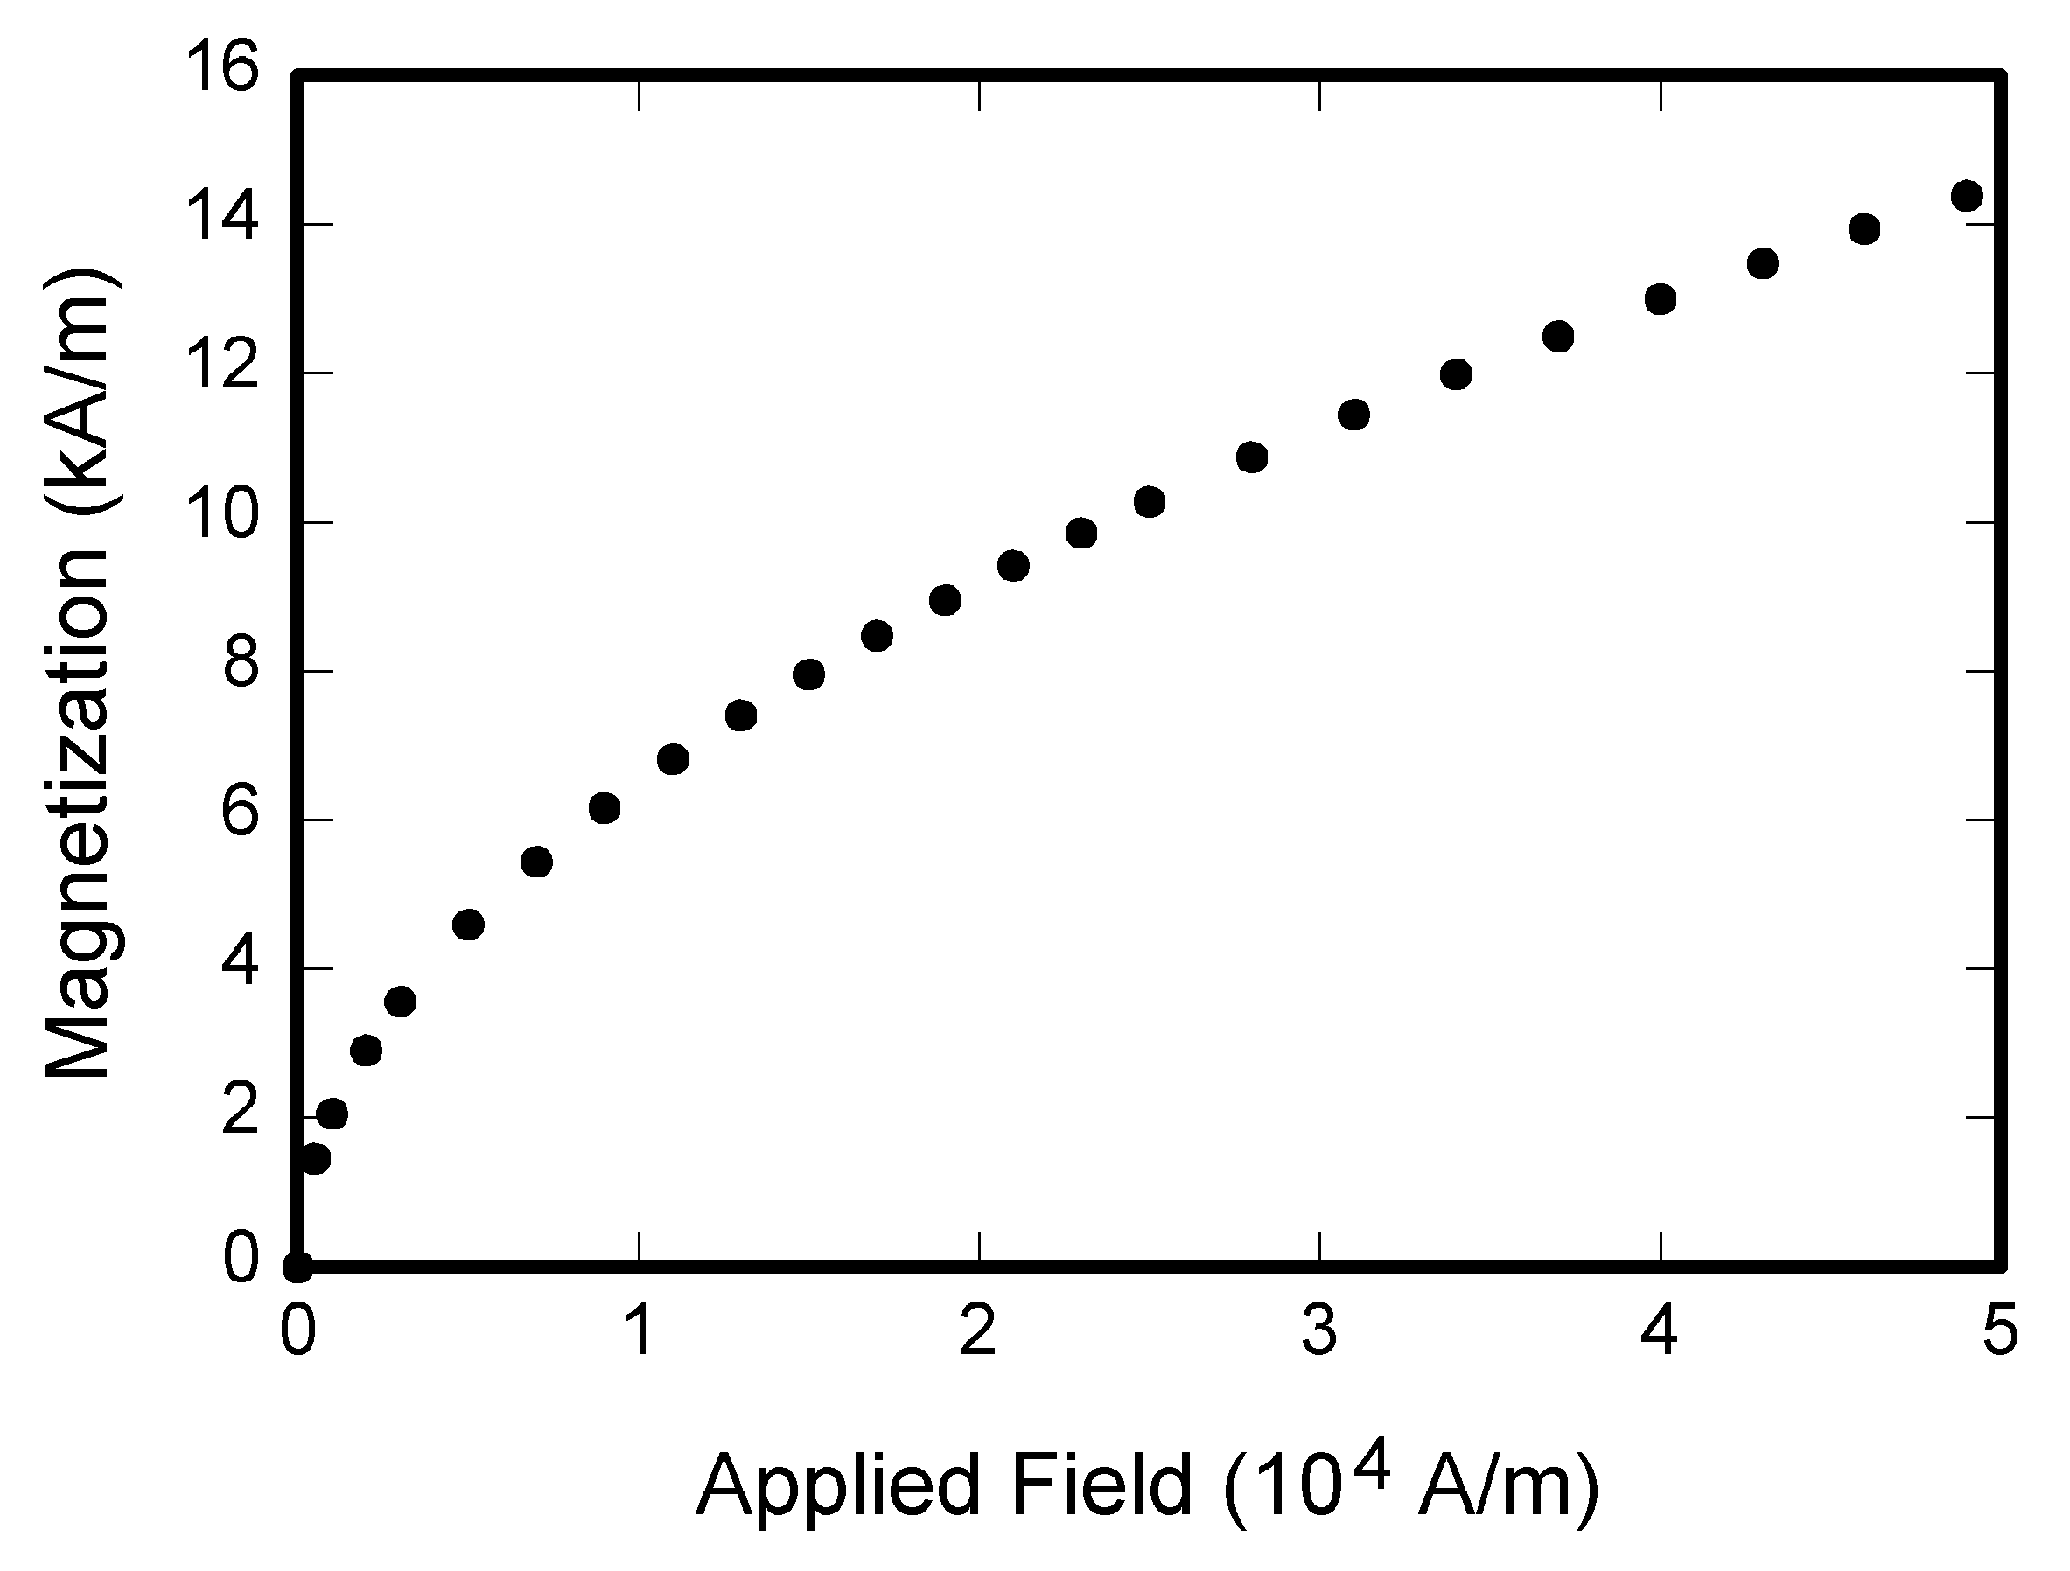
\includegraphics{figures/fig1.png}}
	\caption{Example of a figure caption.}
	\label{fig}
\end{figure}

\section*{References}

Please number citations consecutively within brackets \cite{b1}. The 
sentence punctuation follows the bracket \cite{b2}. Refer simply to the reference 
number, as in \cite{b3}---do not use ``Ref. \cite{b3}'' or ``reference \cite{b3}'' except at 
the beginning of a sentence: ``Reference \cite{b3} was the first $\ldots$''

Number footnotes separately in superscripts. Place the actual footnote at 
the bottom of the column in which it was cited. Do not put footnotes in the 
abstract or reference list. Use letters for table footnotes.

Unless there are six authors or more give all authors' names; do not use 
``et al.''. Papers that have not been published, even if they have been 
submitted for publication, should be cited as ``unpublished'' \cite{b4}. Papers 
that have been accepted for publication should be cited as ``in press'' \cite{b5}. 
Capitalize only the first word in a paper title, except for proper nouns and 
element symbols.

For papers published in translation journals, please give the English 
citation first, followed by the original foreign-language citation \cite{b6}.

\begin{thebibliography}{00}
\bibitem{b1} X. Li, Y. Chen, Y. Wang, and Z. Li, ``Design and implementation of a chess-playing robot based on image recognition,'' in \textit{Proc. IEEE Int. Conf. Robot. Biomimetics (ROBIO)}, Kuala Lumpur, Malaysia, 2018, pp. 2028--2033.
\bibitem{b2} M. Quigley, K. Conley, B. Gerkey, C. Goodrich, and R. VandeWeghe, ``ROS: an open-source robot operating system,'' in \textit{ICRA Workshop on Open Source Software}, Kobe, Japan, 2009, p. 5.
\bibitem{b3} J. Redmon, S. Divvala, R. Girshick, and A. Farhadi, ``You only look once: Unified, real-time object detection,'' in \textit{Proc. IEEE Conf. Comput. Vis. Pattern Recognit. (CVPR)}, Las Vegas, NV, USA, 2016, pp. 779--788.
\bibitem{b4} Y. Wang, X. Wang, and C. Chen, ``Development of a chess-playing robotic arm using deep reinforcement learning,'' in \textit{Proc. IEEE Int. Conf. Robot. Autom. (ICRA)}, Paris, France, 2020, pp. 5314--5319.
\bibitem{b5} Kinova Robotics, ``Kortex ROS packages,'' 2020, gitHub repository. [Online]. Available: https://github.com/Kinovarobotics
\bibitem{b6} S. J. Russell and P. Norvig, \textit{Artificial Intelligence: A Modern Approach}, 4th ed., Pearson, 2020.
\bibitem{b7} M. Young, The Technical Writer's Handbook. Mill Valley, CA: University Science, 1989.
\bibitem{b8} D. P. Kingma and M. Welling, ``Auto-encoding variational Bayes,'' 2013, arXiv:1312.6114. [Online]. Available: https://arxiv.org/abs/1312.6114
\bibitem{b9} R. Nicole, ``Title of paper with only first word capitalized,'' J. Name Stand. Abbrev., in press.
\bibitem{b10} ``Treatment episode data set: discharges (TEDS-D): concatenated, 2006 to 2009.'' U.S. Department of Health and Human Services, Substance Abuse and Mental Health Services Administration, Office of Applied Studies, August, 2013, DOI:10.3886/ICPSR30122.v2
\bibitem{b11} K. Eves and J. Valasek, ``Adaptive control for singularly perturbed systems examples,'' Code Ocean, Aug. 2023. [Online]. Available: https://codeocean.com/capsule/4989235/tree
\end{thebibliography}



\end{document}
